\documentclass[11pt]{article}
\usepackage[margin=1in]{geometry}
\usepackage{amsmath,amssymb}
\usepackage{enumitem}
\usepackage{booktabs}
\usepackage{xcolor}
\usepackage{listings}
\usepackage{graphicx}

\setlength{\parindent}{0pt}
\setlength{\parskip}{4pt}
\setlist[enumerate]{label=(\alph*), leftmargin=*, itemsep=8pt}

\lstset{
  language=R,
  basicstyle=\ttfamily\small,
  keywordstyle=\color{blue!70!black},
  commentstyle=\color{gray},
  frame=single,
  rulecolor=\color{gray!60},
  backgroundcolor=\color{gray!6},
  xleftmargin=4pt, xrightmargin=4pt,
  aboveskip=6pt, belowskip=4pt,
  showstringspaces=false,
  columns=fullflexible,
  keepspaces=true
}

\title{STT 465 -- Homework 3: Normal Models, Prior Choice, and Unknown Variance}
\author{Mihir Patel}
\date{October 30, 2026}

\begin{document}
\maketitle

%==================================================================
\section*{Question 1: Normal Model with Known Variance}

\[
X_1,\dots,X_n \mid \mu \sim N(\mu, \sigma^2), \qquad \mu \sim N(\mu_0, \tau_0^2), \qquad \bar{x} = \frac{1}{n}\sum x_i.
\]

\begin{enumerate}
\item Want to show $\mu \mid x \sim N(\mu_n, \tau_n^2)$ with
\[
\tau_n^2 = \left(\frac{1}{\tau_0^2} + \frac{n}{\sigma^2}\right)^{-1}, \qquad
\mu_n = \tau_n^2\left(\frac{\mu_0}{\tau_0^2} + \frac{n\bar{x}}{\sigma^2}\right).
\]
Likelihood and prior kernels:
\[
L(\mu \mid x) \propto \exp\left[-\frac{1}{2\sigma^2}\sum (x_i - \mu)^2\right], \qquad
\pi(\mu) \propto \exp\left[-\frac{1}{2\tau_0^2}(\mu - \mu_0)^2\right]
\]
\[
\pi(\mu \mid x) \propto \exp\left[-\frac{1}{2}\left(\frac{\sum (x_i-\mu)^2}{\sigma^2} + \frac{(\mu-\mu_0)^2}{\tau_0^2}\right)\right]
\]
Expanding,
\[
\sum (x_i - \mu)^2 = \sum x_i^2 - 2n\bar{x}\mu + n\mu^2, \qquad
(\mu - \mu_0)^2 = \mu^2 - 2\mu_0\mu + \mu_0^2,
\]
and dropping terms without $\mu$,
\[
\pi(\mu \mid x) \propto \exp\left[-\frac{1}{2}\left(\left(\frac{n}{\sigma^2} + \frac{1}{\tau_0^2}\right)\mu^2 - 2\left(\frac{n\bar{x}}{\sigma^2} + \frac{\mu_0}{\tau_0^2}\right)\mu\right)\right]
= \exp\left\{-\frac{1}{2\tau_n^2}\left(\mu^2 - 2\mu\mu_n\right)\right\}
\]
which is the kernel of $N(\mu_n, \tau_n^2)$, so
\[
\boxed{\frac{1}{\tau_n^2} = \frac{1}{\tau_0^2} + \frac{n}{\sigma^2}}, \qquad
\mu_n = \tau_n^2\left(\frac{\mu_0}{\tau_0^2} + \frac{n\bar{x}}{\sigma^2}\right).
\]
The posterior precision is the prior precision plus the data precision.

\item Want $\mu_n = w\bar{x} + (1-w)\mu_0$, $w \in (0,1)$.
\[
\mu_n = \frac{\dfrac{\mu_0}{\tau_0^2} + \dfrac{n\bar{x}}{\sigma^2}}{\dfrac{1}{\tau_0^2} + \dfrac{n}{\sigma^2}}
= \frac{n/\sigma^2}{1/\tau_0^2 + n/\sigma^2}\,\bar{x} + \frac{1/\tau_0^2}{1/\tau_0^2 + n/\sigma^2}\,\mu_0
\]
\[
\boxed{\mu_n = w\bar{x} + (1-w)\mu_0}, \qquad
\boxed{w = \frac{n/\sigma^2}{1/\tau_0^2 + n/\sigma^2} = \frac{n\tau_0^2}{\sigma^2 + n\tau_0^2}}
\]
The weight $w$ is our data precision / total precision. Since both precisions are positive, $0 < w < 1$.

If $\dfrac{n}{\sigma^2} > \dfrac{1}{\tau_0^2}$, $w$ is closer to 1 and posterior mean is closer to $\bar{x}$.

If prior precision $\dfrac{1}{\tau_0^2}$ is bigger, then $w$ is closer to 0 and our posterior mean is closer to $\mu_0$.

\item $X_f \mid \mu \sim N(\mu, \sigma^2)$ and $\mu \mid x \sim N(\mu_n, \tau_n^2)$.
\[
p(x_f \mid x) = \int p(x_f \mid \mu)\,\pi(\mu \mid x)\,d\mu
\]
Write $X_f = \mu + \varepsilon_f$ with $\varepsilon_f \sim N(0, \sigma^2)$ independent of $\mu$, so $X_f \mid x$ is normal (sum of independent normals). Then
\[
E[X_f \mid x] = E\big[E[X_f \mid \mu, x] \mid x\big] = E[\mu \mid x] = \mu_n
\]
\[
\text{Var}(X_f \mid x) = E\big[\text{Var}(X_f \mid \mu, x) \mid x\big] + \text{Var}\big(E[X_f \mid \mu, x] \mid x\big) = \sigma^2 + \tau_n^2
\]
\[
\boxed{X_f \mid x \sim N(\mu_n,\ \sigma^2 + \tau_n^2)}
\]

\item $n = 16$, $\bar{x} = 5.4$, $\sigma^2 = 4$, $\mu \sim N(4,1)$ so $\mu_0 = 4$, $\tau_0^2 = 1$.

Variance:
\[
\tau_n^2 = \left(\frac{1}{\tau_0^2} + \frac{n}{\sigma^2}\right)^{-1} = \left(1 + \frac{16}{4}\right)^{-1} = \boxed{0.2}
\]
Mean:
\[
\mu_n = \tau_n^2\left(\frac{\mu_0}{\tau_0^2} + \frac{n\bar{x}}{\sigma^2}\right) = 0.2\left(4 + \frac{16(5.4)}{4}\right) = \boxed{5.12}
\]
\[
\boxed{\mu \mid x \sim N(5.12,\ 0.2)}, \qquad
\boxed{X_f \mid x \sim N(5.12,\ 0.2 + 4) = N(5.12,\ 4.2)}
\]

\item $\mu \sim N(0, 1000^2)$ so $\mu_0 = 0$, $\tau_0^2 = 1{,}000{,}000$.
\[
\tau_n^2 = \left(\frac{1}{1{,}000{,}000} + \frac{16}{4}\right)^{-1} \approx \boxed{0.25}
\]
\[
\mu_n = \frac{0 + \dfrac{16(5.4)}{4}}{4.000001} \approx \boxed{5.40}
\]
\[
\boxed{\mu \mid x \sim N(5.40,\ 0.25)}, \qquad \boxed{X_f \mid x \sim N(5.40,\ 4.25)}
\]
The difference is 0.28, this is small since data precision is $16/4 = 4$ vs.\ prior precision of 1. Our data will get 80\% of the weight in part (d) while the diffuse prior gives almost no precision, so both posterior means end up close to $\bar{x} = 5.4$.
\end{enumerate}

%==================================================================
\section*{Question 2: Prior Choice and Reparameterization}

\begin{enumerate}
\item $P(10 \le \mu \le 50) \approx 0.95$.
\[
\mu_0 = \frac{10 + 50}{2} = \boxed{30}, \qquad 30 - 2\tau_0 = 10 \;\Rightarrow\; 20 = 2\tau_0 \;\Rightarrow\; \boxed{\tau_0 = 10}
\]
\[
\boxed{\mu \sim N(30,\ 100)}
\]

\item $\pi(\mu) \propto 1$, $-\infty < \mu < \infty$.

It's improper because no positive constant can normalize this density to integrate to 1, since $\int_{-\infty}^{\infty} 1\,d\mu = \infty$.
\[
\pi(\mu \mid x) \propto L(\mu \mid x)\,\pi(\mu) \propto \exp\left[-\frac{1}{2\sigma^2}\sum_{i=1}^n (x_i - \mu)^2\right]
\]
where $\sum (x_i - \mu)^2 = \sum (x_i - \bar{x})^2 + n(\mu - \bar{x})^2$, and the first term doesn't depend on $\mu$, so
\[
\pi(\mu \mid x) \propto \exp\left[-\frac{n}{2\sigma^2}(\mu - \bar{x})^2\right]
\qquad\Rightarrow\qquad
\boxed{\mu \mid x \sim N\left(\bar{x},\ \frac{\sigma^2}{n}\right)}
\]
The normalizing integral is finite for $n \ge 1$ so the posterior is proper even though the prior is improper:
\[
\int_{-\infty}^{\infty} \exp\left[-\frac{n}{2\sigma^2}(\mu - \bar{x})^2\right] d\mu = \sqrt{\frac{2\pi\sigma^2}{n}} < \infty.
\]

\item $\sigma^2 \sim \text{Unif}(0, 10)$, $\tilde{\sigma} = 1/\sigma^2$. Let $v = \sigma^2$ and $\lambda = \tilde{\sigma}$.
\[
\pi_v(v) = \frac{1}{10}, \qquad v = \frac{1}{\lambda}, \qquad \left|\frac{dv}{d\lambda}\right| = \frac{1}{\lambda^2}
\]
\[
\pi_\lambda(\lambda) = \pi_v(1/\lambda)\left|\frac{dv}{d\lambda}\right| = \frac{1}{10\lambda^2}
\]
Support: $0 < v < 10 \Rightarrow \lambda > \frac{1}{10}$.
\[
\boxed{\pi_{\tilde\sigma}(\tilde\sigma) = \begin{cases} \dfrac{1}{10\,\tilde\sigma^2}, & \tilde\sigma > \dfrac{1}{10} \\[4pt] 0, & \text{otherwise} \end{cases}}
\]

\item $\pi(\tilde\sigma) \propto 1$, $\tilde\sigma > 0$. Let $v = \sigma^2$, $\lambda = 1/v$.
\[
\left|\frac{d\lambda}{dv}\right| = \frac{1}{v^2}, \qquad
\pi_v(v) = \pi_\lambda(1/v)\left|\frac{d\lambda}{dv}\right| \propto \frac{1}{v^2}, \quad v > 0
\]
\[
\boxed{\pi(\sigma^2) \propto \frac{1}{(\sigma^2)^2}, \quad \sigma^2 > 0}
\]
Since $1/(\sigma^2)^2$ isn't constant, it's not equal to a flat prior on variance.

A prior that is flat in 1 parameterization generally becomes nonflat after a nonlinear transformation because of the Jacobian factor. So the parameterization used is what decides which prior we call a flat ``non-informative'' prior.

\item $\pi_J(\lambda) \propto \dfrac{1}{\lambda}$, $\lambda > 0$, and $v = \sigma^2 = 1/\lambda$.
\[
\pi_J(v) = \pi_J(1/v)\left|\frac{d\lambda}{dv}\right| \propto \frac{1}{1/v}\cdot\frac{1}{v^2} = v \cdot \frac{1}{v^2} = \frac{1}{v}
\]
\[
\boxed{\pi_J(\sigma^2) \propto \frac{1}{\sigma^2}, \quad \sigma^2 > 0}
\]
Transforming Jeffreys prior using the Jacobian gives the same prior measure as deriving Jeffreys prior directly in the new parameterization.
\end{enumerate}

%==================================================================
\section*{Question 3: Normal Model with Known Mean}

\[
X_1,\dots,X_n \mid \sigma^2 \sim N(\mu, \sigma^2), \qquad \tilde\sigma = \frac{1}{\sigma^2}, \qquad SS_\mu = \sum (x_i - \mu)^2.
\]
Below, $\lambda = \tilde\sigma$.

\begin{enumerate}
\item
\[
f(x \mid \sigma^2) = (2\pi\sigma^2)^{-n/2}\exp\left[-\frac{1}{2\sigma^2}\sum (x_i - \mu)^2\right]
\]
With $\sigma^2 = 1/\lambda$ and $SS_\mu = \sum (x_i - \mu)^2$,
\[
f(x \mid \lambda) = (2\pi)^{-n/2}\lambda^{n/2}\exp\left[-\frac{\lambda}{2}SS_\mu\right]
\]
\[
\boxed{f(x \mid \tilde\sigma) \propto \tilde\sigma^{n/2}\exp\left[-\frac{\tilde\sigma}{2}SS_\mu\right]}
\]

\item $\lambda \sim \text{Gamma}(a_0, b_0)$, so $\pi(\lambda) \propto \lambda^{a_0 - 1}e^{-b_0\lambda}$.
\[
\pi(\lambda \mid x) \propto \lambda^{n/2}e^{-\lambda SS_\mu/2}\,\lambda^{a_0-1}e^{-b_0\lambda}
= \lambda^{a_0 + n/2 - 1}\exp\left[-\left(b_0 + \frac{SS_\mu}{2}\right)\lambda\right]
\]
\[
\tilde\sigma \mid x \sim \text{Gamma}(a_n, b_n), \qquad
\boxed{a_n = a_0 + \frac{n}{2}, \qquad b_n = b_0 + \frac{SS_\mu}{2}}
\]

\item $\pi_J(\tilde\sigma) \propto \dfrac{1}{\tilde\sigma}$.
\[
\pi_J(\lambda \mid x) \propto \lambda^{n/2}e^{-\lambda SS_\mu/2}\,\lambda^{-1} = \lambda^{n/2 - 1}e^{-SS_\mu\lambda/2}
\]
\[
\boxed{\tilde\sigma \mid x \sim \text{Gamma}\left(\frac{n}{2},\ \frac{SS_\mu}{2}\right)}
\]
Posterior is proper when $n > 0$ and $SS_\mu > 0$.

It's the limiting case as $a_0 \to 0^+$ and $b_0 \to 0^+$: the prior kernel approaches $\lambda^{-1}$ and the posterior parameters approach $\frac{n}{2}$ and $\frac{SS_\mu}{2}$. The Jeffreys prior is improper and Gamma$(0,0)$ is not a proper dist.

\item $n = 10$, $\mu = 5$, $SS_\mu = 18$, so $\frac{n}{2} = 5$, $\frac{SS_\mu}{2} = 9$.

Gamma$(2,1)$ prior:
\[
a_n = 2 + 5 = 7, \qquad b_n = 1 + 9 = 10
\]
\[
\boxed{\tilde\sigma \mid x \sim \text{Gamma}(7, 10)}, \qquad \boxed{E[\tilde\sigma \mid x] = \frac{7}{10} = 0.7}
\]
Jeffreys prior:
\[
\boxed{\tilde\sigma \mid x \sim \text{Gamma}(5, 9)}, \qquad \boxed{E[\tilde\sigma \mid x] = \frac{5}{9} \approx 0.556}
\]

\item $\tilde\sigma \mid x \sim \text{Gamma}(a_n, b_n)$ and $X_f \mid \lambda \sim N(\mu, 1/\lambda)$.

Integrating $\lambda$ out,
\[
p(x_f \mid x) \propto \left[1 + \frac{(x_f - \mu)^2}{2b_n}\right]^{-(a_n + 1/2)}
\]
Matching to the $t$ kernel $\left[1 + \dfrac{(x_f - m)^2}{\nu s^2}\right]^{-(\nu+1)/2}$:
\[
\boxed{\nu = 2a_n, \qquad m = \mu, \qquad s = \sqrt{\frac{b_n}{a_n}}}
\]
Using the conjugate posterior from (d), $a_n = 7$, $b_n = 10$, $\mu = 5$:
\[
\boxed{X_f \mid x \sim t_{14}\left(\text{location} = 5,\ \text{scale} = \sqrt{\tfrac{10}{7}}\right)}, \qquad \text{degrees of freedom} = 14
\]
\end{enumerate}

%==================================================================
\section*{Question 4: Normal Model with Unknown Mean and Variance}

\[
X_1,\dots,X_n \mid \mu, \sigma^2 \sim N(\mu, \sigma^2), \qquad
\mu \mid \sigma^2 \sim N\left(\mu_0, \frac{\sigma^2}{p_0}\right), \qquad
\sigma^2 \sim IG\left(\frac{\nu_0}{2}, \frac{SS_0}{2}\right),
\]
\[
SS = \sum (x_i - \bar{x})^2.
\]

\begin{enumerate}
\item Want to show
\[
p_n = p_0 + n, \qquad \mu_n = \frac{p_0\mu_0 + n\bar{x}}{p_0 + n}, \qquad \nu_n = \nu_0 + n, \qquad
SS_n = SS_0 + SS + \frac{p_0 n}{p_0 + n}(\bar{x} - \mu_0)^2.
\]
Using $\sum (x_i - \mu)^2 = SS + n(\mu - \bar{x})^2$,
\[
L(\mu, \sigma^2 \mid x) \propto (\sigma^2)^{-n/2}\exp\left[-\frac{SS + n(\mu - \bar{x})^2}{2\sigma^2}\right]
\]
Multiplying by the prior,
\[
\pi(\mu, \sigma^2 \mid x) \propto (\sigma^2)^{-\left(\frac{\nu_0 + n}{2} + \frac{3}{2}\right)}
\exp\left[-\frac{SS_0 + SS + n(\mu - \bar{x})^2 + p_0(\mu - \mu_0)^2}{2\sigma^2}\right]
\]
Completing the square,
\[
n(\mu - \bar{x})^2 + p_0(\mu - \mu_0)^2 = (p_0 + n)(\mu - \mu_n)^2 + \frac{p_0 n}{p_0 + n}(\bar{x} - \mu_0)^2
\]
So the posterior kernel is
\[
\underbrace{(\sigma^2)^{-1/2}e^{-p_n(\mu - \mu_n)^2/(2\sigma^2)}}_{\text{normal in } \mu}\;
\underbrace{(\sigma^2)^{-(\nu_n/2 + 1)}e^{-SS_n/(2\sigma^2)}}_{\text{inverse gamma in } \sigma^2}
\]
\[
\boxed{\mu \mid \sigma^2, x \sim N\left(\mu_n, \frac{\sigma^2}{p_n}\right), \qquad
\sigma^2 \mid x \sim IG\left(\frac{\nu_n}{2}, \frac{SS_n}{2}\right)}
\]
which is still normal-inverse-gamma with the updated quantities above.

\item
\[
\mu_n = \frac{p_0}{p_0 + n}\mu_0 + \frac{n}{p_0 + n}\bar{x}
\]
$\mu_n$ is the weighted avg of our prior mean and sample mean. $p_0$ acts like a prior sample size for estimating $\mu$, so big $p_0$ gives more weight to prior mean.

\item
\[
SS_n = SS_0 + SS + \frac{p_0 n}{p_0 + n}(\bar{x} - \mu_0)^2
\]
$SS_0$ is the prior contribution to our sum of squares parameter, while $SS$ is $\sum (x_i - \bar{x})^2$ which measures the variation of the observations around their sample mean, and $\frac{p_0 n}{p_0 + n}(\bar{x} - \mu_0)^2$ is the disagreement between prior mean vs.\ sample mean.

The difference between prior and sample mean is squared, so when they strongly disagree this term gets big, which increases our posterior variance scale.

\item $p_0 = 4$, $\mu_0 = 10$, $\nu_0 = 6$, $SS_0 = 30$, $n = 8$, $\bar{x} = 12$, $SS = 42$.
\[
\boxed{p_n = 4 + 8 = 12}
\]
\[
\boxed{\mu_n = \frac{4(10) + 8(12)}{12} = \frac{34}{3} \approx 11.333}
\]
\[
\boxed{\nu_n = 6 + 8 = 14}
\]
\[
\boxed{SS_n = 30 + 42 + \frac{4(8)}{12}(12 - 10)^2 = \frac{248}{3} \approx 82.667}
\]
\[
\boxed{\mu \mid \sigma^2, x \sim N\left(\frac{34}{3}, \frac{\sigma^2}{12}\right)}, \qquad
\boxed{\sigma^2 \mid x \sim IG\left(7, \frac{124}{3}\right)}
\]

\item
\[
\mu \mid x \sim t_{\nu_n}\left(\mu_n, \sqrt{\frac{SS_n}{p_n\nu_n}}\right), \qquad
\sqrt{\frac{SS_n}{p_n\nu_n}} = \sqrt{\frac{248/3}{12(14)}} = \sqrt{\frac{31}{63}} \approx 0.701
\]
\[
\boxed{\mu \mid x \sim t_{14}\left(\text{location} = \frac{34}{3},\ \text{scale} = \sqrt{\tfrac{31}{63}}\right)}
\]
Since $\sigma^2$ is unknown we have to integrate it out of $\mu \mid \sigma^2, x \sim N(\mu_n, \sigma^2/p_n)$ using its inverse gamma posterior. Averaging normals over an inverse gamma variance gives a $t$, which has heavier tails than a normal because it accounts for our uncertainty about $\sigma^2$.
\end{enumerate}

%==================================================================
\section*{Question 5: Posterior Simulation and Prior Sensitivity}

\[
x = (8.4,\ 10.1,\ 9.7,\ 11.2,\ 10.5,\ 9.1,\ 10.8,\ 11.0,\ 9.6,\ 10.3), \qquad
\mu_0 = 9,\ p_0 = 3,\ \nu_0 = 4,\ SS_0 = 8.
\]

\begin{enumerate}
\item From R (code in part (b)):
\[
\boxed{n = 10, \qquad \bar{x} = 10.07, \qquad SS = 7.001}
\]
\[
p_n = 13, \qquad \mu_n = \frac{3(9) + 10(10.07)}{13} = \frac{127.7}{13} \approx 9.82, \qquad \nu_n = 14
\]
\[
SS_n = 8 + 7.001 + \frac{30}{13}(10.07 - 9)^2 = 17.643
\]
\[
\boxed{\sigma^2 \mid x \sim IG(7,\ 8.82)}, \qquad \boxed{\mu \mid \sigma^2, x \sim N\left(9.82,\ \frac{\sigma^2}{13}\right)}
\]

\item R code used for the simulation:
\begin{lstlisting}
set.seed(2026)

x <- c(8.4, 10.1, 9.7, 11.2, 10.5,
       9.1, 10.8, 11.0, 9.6, 10.3)

n <- length(x)
xbar <- mean(x)
SS <- sum((x - xbar)^2)
B <- 50000

simulate_posterior_with_50000 <- function(mu0, p0, nu0, SS0) {
  pn <- p0 + n
  mun <- (p0 * mu0 + n * xbar) / pn
  nun <- nu0 + n
  SSN <- SS0 + SS + p0 * n / pn * (xbar - mu0)^2

  sigma2 <- 1 / rgamma(
    B, shape = nun / 2, rate = SSN / 2
  )

  mu <- rnorm(
    B, mean = mun, sd = sqrt(sigma2 / pn)
  )

  list(mu = mu, sigma2 = sigma2)
}

original <- simulate_posterior_with_50000(
  mu0 = 9, p0 = 3, nu0 = 4, SS0 = 8
)

#part c estimating the posterior
mean(original$mu)
mean(original$mu > 10)
quantile(original$mu, c(0.025, 0.975))

#part d with original priors
mean(original$sigma2)
quantile(original$sigma2, c(0.025, 0.975))

par(mfrow = c(1, 2))

plot(density(original$mu),
     main = "Posterior density of mu",
     xlab = expression(mu))

plot(density(original$sigma2, from = 0),
     main = "Posterior density of variance",
     xlab = expression(sigma^2))

#part e with weak priors
weak <- simulate_posterior_with_50000(
  mu0 = 0, p0 = 0.01,
  nu0 = 0.01, SS0 = 0.01
)

mean(weak$mu)
mean(weak$mu > 10)
quantile(weak$mu, c(0.025, 0.975))

mean(weak$sigma2)
quantile(weak$sigma2, c(0.025, 0.975))
\end{lstlisting}

\item
\[
\boxed{E[\mu \mid x] \approx 9.822}, \qquad \boxed{P(\mu > 10 \mid x) \approx 0.2866}, \qquad
\boxed{95\% \text{ CI for } \mu: (9.1619,\ 10.4869)}
\]
28.7\% is our posterior probability that $\mu > 10$.

\item
\[
\boxed{E[\sigma^2 \mid x] \approx 1.4678}, \qquad \boxed{95\% \text{ CI for } \sigma^2: (0.677,\ 3.1288)}
\]
\begin{center}
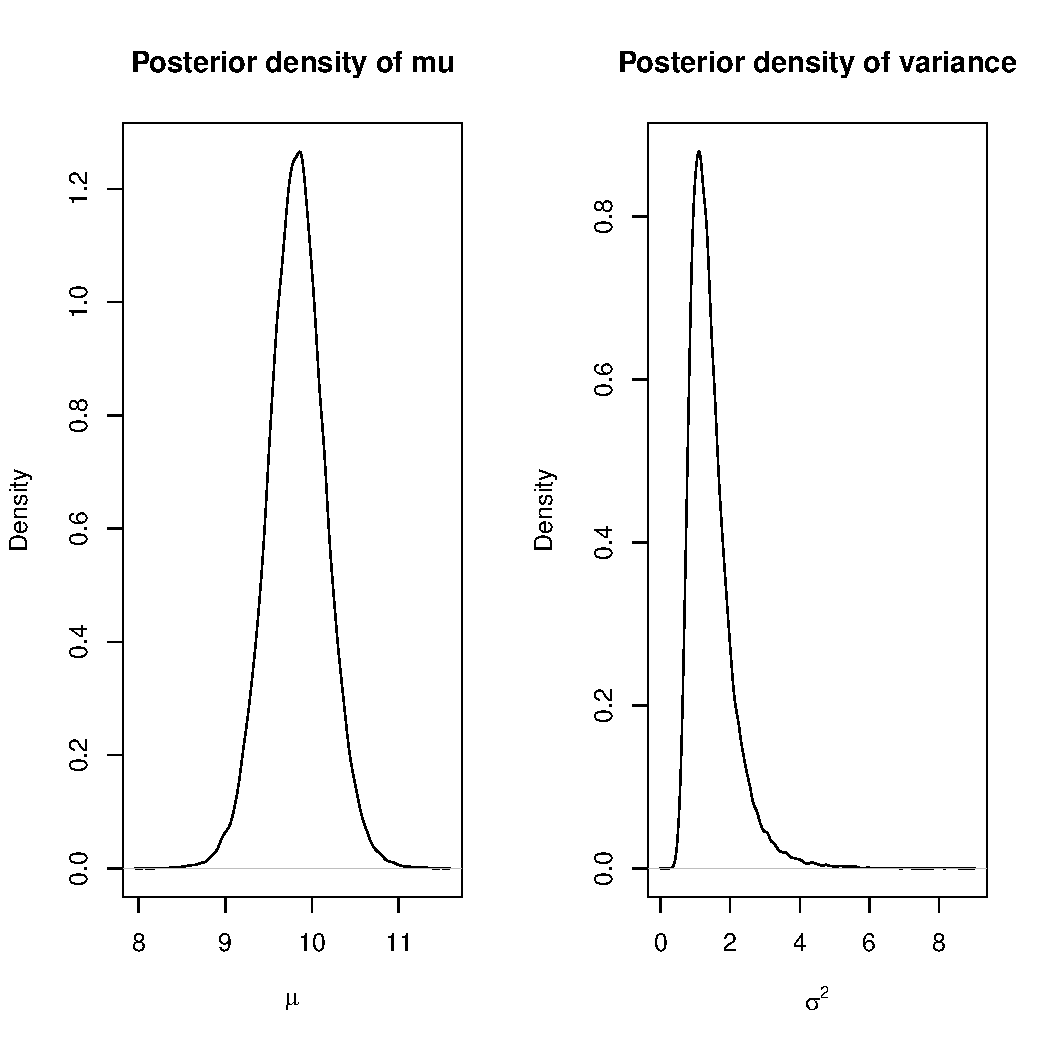
\includegraphics[width=0.6\textwidth]{Rplots.pdf}
\end{center}

\item Weak prior: $\mu_0 = 0$, $p_0 = 0.01$, $\nu_0 = 0.01$, $SS_0 = 0.01$.
\[
p_n = 10.01, \qquad \mu_n = 10.0599, \qquad \nu_n = 10.01
\]
\[
SS_n = 0.01 + 7.001 + \frac{0.01(10)}{10.01}(10.07 - 0)^2 = 8.0240
\]
\[
\boxed{\sigma^2 \mid x \sim IG(5.005,\ 4.012)}, \qquad \boxed{\mu \mid \sigma^2, x \sim N\left(10.0599,\ \frac{\sigma^2}{10.01}\right)}
\]
From the simulation:
\begin{center}
\begin{tabular}{lcc}
\toprule
 & Original prior & Weak prior \\
\midrule
$E[\mu \mid x]$ & 9.8222 & 10.0588 \\
$P(\mu > 10 \mid x)$ & 0.2866 & 0.5812 \\
95\% CI for $\mu$ & (9.1619, 10.4869) & (9.4232, 10.6856) \\
$E[\sigma^2 \mid x]$ & 1.4678 & 1.0015 \\
95\% CI for $\sigma^2$ & (0.6777, 3.1288) & (0.3943, 2.4719) \\
\bottomrule
\end{tabular}
\end{center}
Under the original prior the posterior mean is 9.82 and under the weak prior it's 10.06, so the original prior pulls $\mu$ down toward $\mu_0 = 9$. The credible intervals are about the same width but the original one is shifted down by about 0.24.

The data are fairly strong since $n = 10$ vs.\ $p_0 = 3$, so the data gets $10/13 \approx 77\%$ of the weight on the mean, but the prior still has a noticeable effect (it moves $P(\mu > 10 \mid x)$ from 0.58 to 0.29). With the weak prior the posterior is basically just the data, $\mu_n \approx \bar{x}$.
\end{enumerate}

\end{document}
